\vsssub
\subsubsection{The Restart File Processor} \label{sec:ww3uprstr}
\vsssub

\proddefH{ww3\_uprstr}{ww3uprstr}{ww3\_uprstr.ftn}
\proddeff{Input}{ww3\_uprstr.inp}{Traditional configuration file.}{10} (App.~\ref{sec:config221})
\proddefa{mod\_def.ww3}{Model definition file.}{20}
\proddefa{restart.ww3}{Restart File}{ }
\proddefa{XXXX.grbtxt}{SWH Analysis file in grbtxt format.}{123}
\proddeff{Output}{restart001.ww3}{Updated restart file.}{ }

\vspace{\baselineskip} 

\paragraph{Introduction \newline } 

The majority of the observations for the sea surface wave field is 
observations of the diagnostic variable: Significant Wave Height (SWH). 
Therefore, the wave data assimilation (WDA) often takes space in the SWH 
space and subsequently this information has to be transfered to the 
prognostic space, wave spectrum (WS) to be imposed as boundary and/or 
initial condition (BIC). 

\subparagraph{Purpose of the \textbf{ww3\_uprstr}  \newline } Redistribution of 
the energy from the analysis of the SWH field to the field of WS saved
in the restart file. 

\subparagraph{Core algorithm \newline } 
The \textbf{ww3\_uprstr} sets the SWH of the background spectra equal to 
the SWH of the analysis and modifies the shape of the spectrum according 
to the user's prescibed spectrum shape. The \textbf{ww3\_uprstr} has been  
implemented as an extension of the restart reader and it requires as inputs: 
the restart file, the SWH of the analysis, and the \textbf{ww3\_uprstr.inp} 
(see above) with the user's defined options; additional files may be
required in order to reduce the calculations on the fly.

\paragraph{How to Use the ww3\_uprstr \newline}
To use the \textbf{ww3\_uprstr}, the users have to follow the same logic 
as for all the WAVEWATCH III programs. In summary: 

\begin{enumerate}
   \item \textbf{Download the source code} \newline
   The \textbf{ww3\_uprstr} source code is included to the official WAVEWATCH III
   release, starting with the version x.xx.
   \item \textbf{Compile the code} \newline
   The \textbf{ww3\_uprstr} is compiled the same way as all the auxiliary programs 
   of WAVEWATCH III, see the appropriate section of the manual. For debugging outputs, 
   use the  \textbf{T} flag at the switch file.
   \item \textbf{Test the executable} \newline
   The regression test \textbf{ww3\_ta1} can be used for testing the different 
   options of \textbf{ww3\_uprstr}.  
   \item \textbf{Run the ww3\_uprstr} \newline
   Description of steps to run the \textbf{ww3\_uprstr}:
   \begin {description}
      \item{Required Input files: \newline}
      \begin{itemize}
         \item \textbf{Restart file.} This file has been created by WW3 during the hindcast run
         of the model or during the previous cycle.
         Expected filename: \textbf{restart.ww3}.
         \item \textbf{mod\_def.ww3}
         \item \textbf{ww3\_uprstr.inp.} This is the input file for the \textbf{ww3\_uprstr}. 
         The users have to define i. the date of the assimilation, ii. the method of energy
         redistribution and iii. depending on the method: a percentage or an inputfile.
         \item \textbf{Input file of analysis.} The file can have any name, but the suffix 
         defines the reader used for importing the data. For the majority of options, the reader supports only
         \textbf{grbtxt} format. This is a text file created with wgrib2 from the grib2 file 
         of the analysis and it has the following structure:\newline

         \begin{tabular}{|c|}
            \hline
            NX NY       \\
            VAL0001     \\
            VAL0002     \\
            ...         \\
            VAL(NX*NY)  \\
            \hline   
          \end{tabular}
    \newline
    \item To run the executable: \newline 
          \textgreater \$EXE/ww3\_uprstr \newline 
          If all the inputs are correctly prepared, a new restart file 
          (\textbf{restart001.ww3}) will be created. The \textbf{ww3\_uprstr} 
          exports the updated spectra in the same format as the restart.ww3. 
          To be applied as BIC for the initialization of the next prediction cycle,
          it has to be renamed: \newline
          \textgreater mv \textbf{restart001.ww3} \textbf{restart.ww3}) \newline      
          The updated restart file is used as normally.
      \end{itemize}
   \end{description}
   
   \noindent\fbox{
      \parbox{\textwidth}{
         \textbf{Tips}
         \begin{itemize}
            \item The restart file has to be created with the same WW3 version as 
         the \textbf{ww3\_uprstr}; there is not backwards compatibility.
            \item The starting time of the assimilation defined at \textbf{ww3\_uprstr.inp}
         has to be the same with the time at the restart file.
            \item By using the \textbf{T}, the \textbf{ww3\_uprstr.inp} exports the fields of 
         SWH from the background restart file, the analysis and of the updated restart file.
         In addition, the spectra from the restart files before and after and the update are
         exported as text files.  
         \end{itemize}
         }
   }
\end{enumerate}
 
\subparagraph{Update method \newline}
The users have to define the update algorithm of their choice at the
\textbf{ww3\_uprstr.inp}. The options for updating the restart file are defined at the 
ww3\_uprstr.inp with the flag UPD[N], where N could be 0F, 0C, 1, 2,... 
For UPDN, with N \textless 2, the same correction is applied to the whole grid;
Expected input: PRCNTG, as defined at fac.
For UPDN, with N \textgreater 1 each gridpoint has its own update factor and the input
is at grb2txt format. For more details about the current implementation see the 
~\ref{fig:uprstrflowchart}.

\begin{figure} \begin{center}
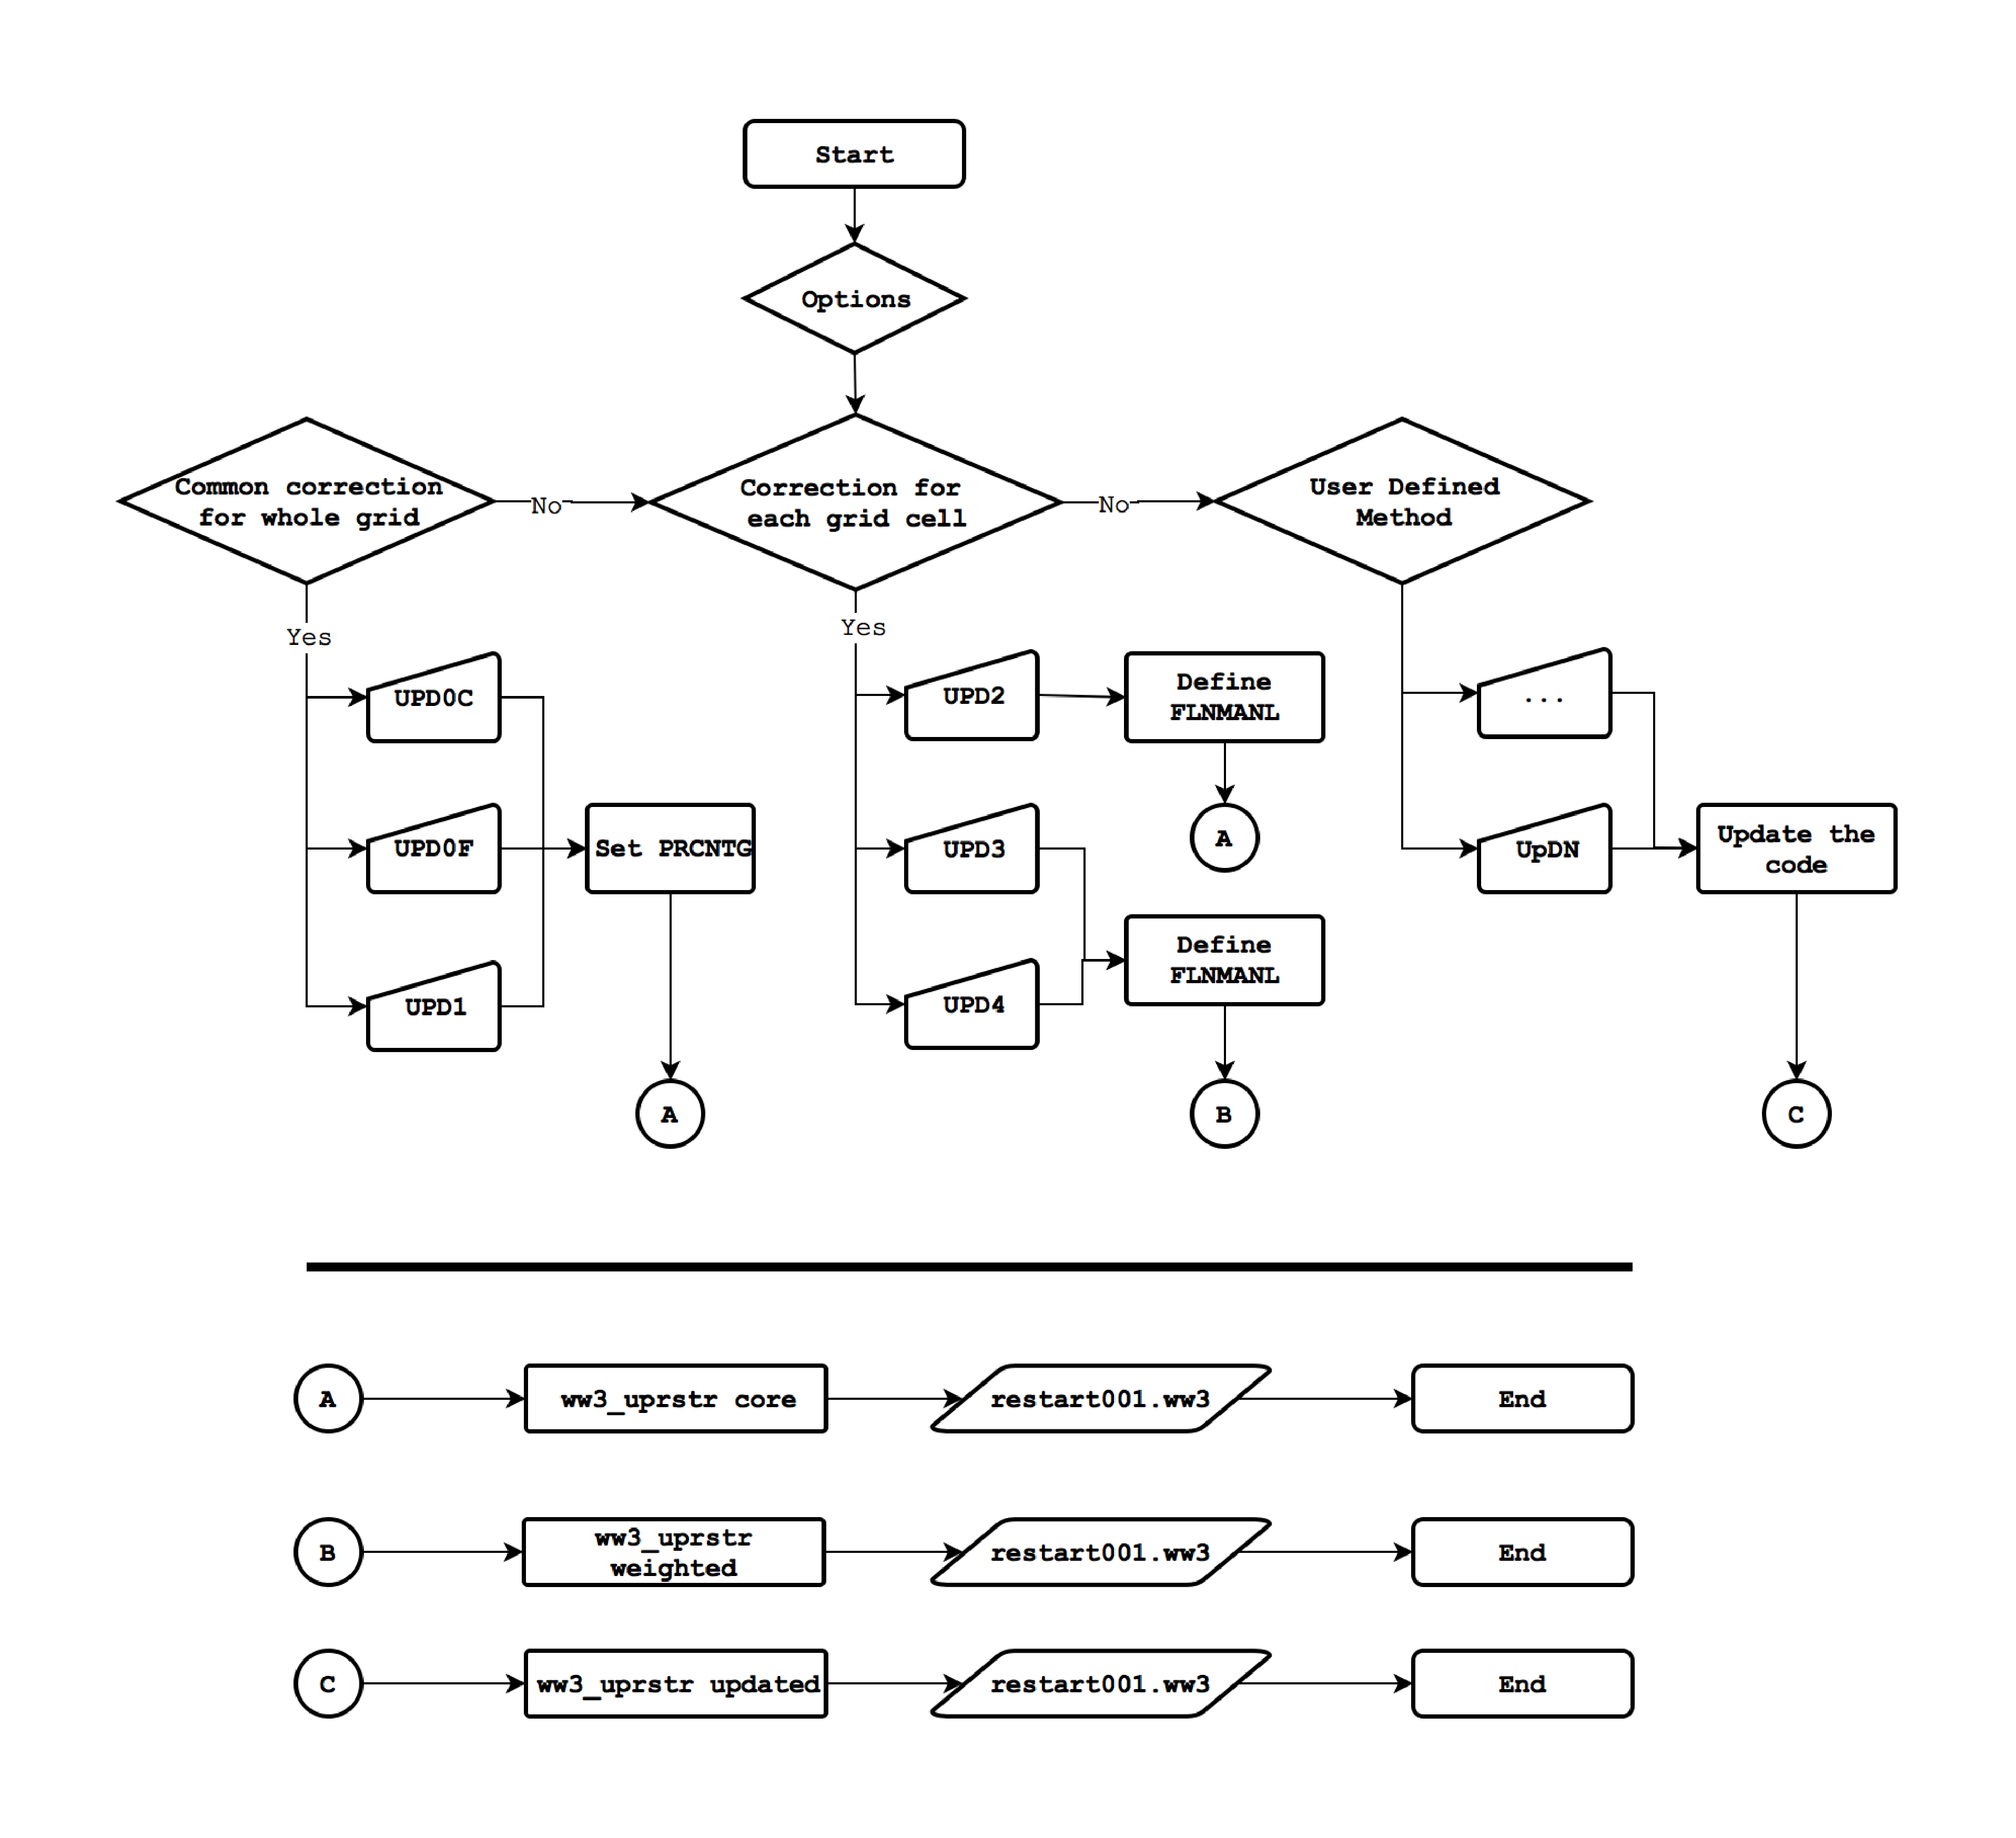
\includegraphics[width=0.9\textwidth]{./run/uprstr.eps}
\caption{Flowchart of the implemented methods for updating the wave spectra at the WW3 
restart file. Additional methods can be implemented by adding UPD options to the namelist.}
\label{fig:uprstrflowchart} \botline
\end{center}
\end{figure}

The following UPD options are available:
\begin{enumerate} 
   \item UPD0C:: \textbf{ELIMINATED from version x.xx} Option 0C  All the spectra are 
   updated with a constant: \newline
      \(fac=(SWH\_Bckg-SWH\_Anl)/SWH\_Anl \).
   \item UPD0F:: Option 0F  All the spectra are updated with a constant: \newline 
      \(fac=SWH\_Anl/SWH\_Bckg \).
   \item UPD1 ::  \textbf{ELIMINATED from version x.xx} Option 1  The fac(x,y,frq,theta), 
   is weighted according to the \% of energy at each spectral bin; fac the same as UPDOF.
   \item UPD2 :: Option 2   The fac(x,y,frq,theta), is calculated at each grid point 
   according to SWH\_Bckg and SWH\_Anl
   \item UPD3 :: Option 3   The update factor is a surface with the shape of 
   the background spectrum. 
   \item UPD4 :: [NOT INCLUDED in the current version, just keeping the spot]
   Option 4  The generalization of the UPD3. The update factor is the sum of surfaces 
   which are applied on the background spectrum. The algorithm requires the mapping 
   of each partition on the individual spectra; the map is used to determine the weighting 
   surfaces.
   \item UPD5 :: Option 5   Corrections are calculated as per UPD2 but are
   applied to wind-sea parts of the spectrum only when wind-sea
   is the dominant component, otherwise the whole spectrum is
   corrected. Required inputs are the the Analysis Hs field plus 
   background wind speed and direction. To include the wind data it is recommended
   to run code built with the WRST switch.
   \item UPD6 :: Option 6   Corrections are calculated as per UPD5 but wind-sea
   components are also shifted in frequency space using Toba (1973).
   Required inputs are the the Analysis Hs field plus background wind speed and direction.
   To include the wind data it is recommended to run code built with the WRST switch.
\end{enumerate}

Any additional method for the redistribution of the energy to the WS and correcting 
the associated winds could be added by further extending the input file and adding 
the source code to the \textbf{ww3\_uprstr.ftn}.

\subparagraph{Example \newline}
In this section, an example of the simplest WDA application is discussed.
The figure ~\ref{fig:waveDAflowchart} shows how the \textbf{ww3\_uprstr} 
is used in the framework of a simple wave analysis system. \newline

A WW3 run (from the previous cycle or from the hindcast) provides the
background field of SWH and the corresponding restart file at the appropriate time. 
The format of the background SWH field has to be compatible with the WDA module inputs.

\begin{figure} \begin{center}
\includegraphics[width=0.9\textwidth]{./run/waveDA.eps}
\caption{Flowchart of simplified wave data assimilation system, 
showing the role of the {ww3\_uprstr}, the required input files,
and the resulted output of the updated restart file.}
\label{fig:waveDAflowchart} \botline
\end{center}
\end{figure}

The WDA module uses the background field and the available observations
for the time of analysis, produces the analysis and exports 
the field of SWH in grbtxt format (\textbf{XXXX.grbtxt}) .

The analysis file, the \textbf{mod\_def.ww3}, the \textbf{restart.ww3} file and 
the \textbf{ww3\_uprstr.inp} are the input files for the \textbf{ww3\_uprstr}. 
If all the options and input files are correctly prepared, it takes approxmately 
one minute to update a grid of 260000 grid nodes and generate the output on a single processor. 
The updated restart file has to be renamed, at the expected file name, in the case of this
example to \textbf{restart.ww3}. \newline  

   \noindent\fbox{
      \parbox{\textwidth}{
      \textbf{Note: }
      All \ncep's WDA systems use GRIB2 format, thereore there is always an intermediate
      step to transfer the grib files to the appropriate format. The used software is WGRIB2 
      and more information can be retrieve from the 
      \href{http://www.cpc.ncep.noaa.gov/products/wesley/wgrib2} {official website}.       
      }
   }

%\paragraph{How to Update the ww3\_uprstr \newline}
%Add data readers, mainly for machine independent binary data and wgrib2.

\pb
